\chapter[Fundamentação Teórica]{Fundamentação Teórica}\label{cap2}

Neste capítulo estão as pesquisas e todo o embasamento teórico referente a literatura acerca de trabalhos já desenvolvidos que dão suporte e direcionam o tema deste trabalho. As seções contidas neste capítulo abordam temas referentes ao surgimento e crescimento dos \textit{audiobooks} bem como os formatos existentes, acessibilidade, pessoas com deficiência visual e suas dificuldades e limitações, formato de áudio e também traz uma contextualização sobre a viabilidade e aceitação do tema proposto.

\section{Terminologia}

Segundo Romeu Kasumi Sassaki, ``a construção de uma verdadeira sociedade inclusiva passa também pelo cuidado com a linguagem'' \cite{sassaki}. Em seu estudo, Sassaki relata sobre a importância da linguagem utilizada pois através dela podemos expressar, seja voluntariamente ou não, o respeito ou a discriminação em relação às pessoas com deficiência. Dentre as terminologias corretas citadas por Sassaki nós podemos utilizar: cego, pessoa cega, pessoa com deficiência visual, deficiente visual, cegueira e baixa visão. A deficiência visual diferencia-se entre deficiência visual parcial, quando a pessoa possui baixa visão, e cegueira, quando a deficiência visual é total \cite{sassaki}.

O termo portador de deficiência foi largamente utilizado no Brasil entre os anos de 1986 e 1996. No entanto, em 2003, Sassaki disse que o uso é incorreto visto que a deficiência não é uma coisa que portamos ou não como um documento de identidade, por exemplo, e sugere a terminologia pessoa com deficiência como correto \cite{sassaki}. Em 2006, a Assembleia da ONU aprovou a Convenção Sobre os Direitos das Pessoas com Deficiência onde, assinada pelo Brasil em 2007 e ratificada pelo Congresso Nacional em 2008, acaba por oficializar o termo pessoa com deficiência em seu próprio título \cite{bengalalegal}.

A Câmara dos Deputados utiliza e orienta as pessoas a utilizarem o termo hoje mundialmente aceito, a saber: pessoa com deficiência. Diz também que os termos cego e surdo podem ser utilizados \cite{camara}.

\section{Audiobooks}

Podemos dizer que \textit{audiobook} é a versão em áudio de livros impressos. Também conhecido como ``livro falado'', o \textit{audiobook} tem sido conhecido aos poucos aqui no Brasil e utilizado como suporte para que pessoas que não possuem o hábito de ler passam a conhecer obras literárias. A partir da leitura do livro feita em voz alta, o conteúdo do livro é gravado e armazenado em formatos diversificados tais como CD, MP3, WMA e Ogg. O controle de qualidade destas gravações estão ligadas principalmente ao formato que está sendo utilizado como suporte. Outros requisitos, não menos importantes, tratam dos narradores e da interpretação que se dá ao personagem, das variações no tom de voz em diálogos bem como os efeitos sonoros produzidos trazendo maior realismo e um maior envolvimento na história ajudando na interpretação  do texto \cite{torrenttitles}.

O audiobook é uma forma inovadora de acesso à leitura \cite{audiobooksuporte}. Mesmo para aquelas pessoas que possuem o hábito de leitura, este hábito vem se perdendo devido ao ritmo acelerado das grandes cidades do mundo de hoje. Por falta de tempo, as pessoas tem feito uso de \textit{audiobooks} para estarem ``lendo'' enquanto passam horas dirigindo em extensos engarrafamentos ou enquanto fazem exercícios físicos \cite{audiobookinovacao}. Isso é possível pois a portabilidade do audiobook em comparação aos livros impressos é muito maior, pois o local não parece importar. Os audiobooks também podem ser utilizados em sala de aula como suporte à alfabetizacão e como instrução de uma segunda língua.

Desde o início da década de 50, a apreciação pela literatura falada vem crescendo e se tornando tradição nos Estados Unidos. Mas foi em 1980 que realmente os audiobooks ganharam corpo. Segundo \cite{teixeira} havia, em 2006, cerca de 30 mil títulos de \textit{audiobooks} nos Estados Unidos disponíveis considerando apenas o site da Audible, companhia da Amazon. No ano de 2014, a companhia possui mais de 150 mil títulos disponíveis para download \cite{audible}. Este número mostra como o mercado de \textit{audiobooks} vem crescendo no mercado norte-americano.

O crescimento do uso de \textit{audibooks} não tem ocorrido apenas nos Estados Unidos. Na Europa, os livros falados também tem ganhado força, sendo mais popular na Alemanha. Neste país, o hábito virou moda na década de 90. Podemos citar o Instituto Goethe que é um instituição sem fins lucrativos que visa a disseminação do idioma e cultura alemã. Eles possuem \textit{streaming} de diversas obras literárias alemãs hospedadas e disponíveis em seu site. Sabe-se que dois eventos populares na Alemanha, a grande Feira Internacional de Livros de Leipzig e o Festival Internacional de Literatura de Berlim, contam com estandes de venda voltados à apresentação de \textit{audiobooks} \cite{dw}.

Oscar Niemeyer, antes mesmo do uso dos CDs, certa vez disse ``Quando quero ler, eu ouço. Pago uma pessoa para gravar os livros em fitas e depois, quando sinto vontade, as coloco para tocar'' \cite{audiobookinovacao}. Aqui no Brasil, o uso de \textit{audiobooks} começou um pouco mais tarde e em um ritmo um pouco mais lento se comparado com Estados Unidos e Europa. No entanto, nos últimos anos os livros falados tem sido cada vez mais utilizados pela população brasileira. O mercado brasileiro tem correspondido a esta nova disseminação cultural \cite{farias}. Isto mostra que a cultura de livros falados no Brasil veio para ficar. Plugme e Audiolivro Editora são editoras que tem investido em audiolivros no Brasil. Em 2008, quando o mercado ainda era considerado tímido, a Plugme registrou uma venda de setecentos livros por mês contra mil livros da Audiolivro \cite{audiobooksuporte}. A Audiolivro conta com mais de 900 títulos. Voltado para a literatura infantil, a editora RHJ reúne mais de 200 publicações e premiações recebidas no exterior tais como \textit{White RAvens} na Alemanha, \textit{Octogone} na França, \textit{BIB Plaque} na Eslováquia, \textit{The Noma Concours} no Japão e \textit{The Ibby Honour List Diploma} no Canadá. A editora RHJ também possui premiações no Brasil \cite{rhj}.

A Universidade Falada é um portal de iniciativa privada que visa difundir cultura pelo Brasil com distribuição de conteúdo em áudio viabilizado pela \textit{Editora Alyá} com preços acessíveis e facilidade para a aquisição. Este projeto conta com mais de mil e trezentos audiolivros e estimam mais de cinco mil horas de áudio disponíveis em formato mp3. \cite{universidadefalada}.

\begin{citacao}
O projeto Universidade Falada® pretende democratizar a cultura. Facilitar o acesso, em formato áudio e audiolivro, a grandes obras da literatura nacional e internacional à população mais afastada dos grandes centros culturais do país. Nossa missão é ajudar pessoas, oferecer conhecimento e cultura. Discutir temas velhos e novos, ensinar e filosofar. Agregar valor ao ser humano. É isso que nós editores, autores e palestrantes desejamos desta empreitada. Nossos preços permitem que qualquer brasileiro com acesso a internet possa adquirir nossos produtos. Sem exceção \cite{universidadefalada}.
\end{citacao}

Em outubro deste ano, a \textit{PublishNews} publicou uma matéria informando a chegada de duas plataformas de audiolivros para smartphones e tablets no mercado brasileiro. A UBook é uma delas e já está disponível para plataforma iOS e Android. Adotando o serviço de subscrição, os usuários possuem acesso ilimitado a mais de mil obras. Segundo os desenvolvedores, cinco dias após seu lançamento, a plataforma já possuia mais de vinte mil usuários. Uma outra alternativa é a TocaLivros que optou pela venda unitária do audiolivro em formato digital \cite{publishnews}. %Lançada em novembro de 2014, a TocaLivros deve chegar a 2.500 obras literárias até o final de 2015 com uma meta de 200 mil usuários \cite{startupi}.

\section{Audiobook e as Pessoas com Deficiência Visual}

Como estrelas que brilham no campo editorial é evidente a popularidade dos audiobooks \cite{printdisable}. No entanto, acessibilidade ainda é um desafio para os publicadores pois os formatos não são totalmente acessíveis \cite{challenge}. Um jornal televisivo de média audiência levou ao ar uma matéria que trata da experiência de pessoas com deficiência visual no uso da Internet. Um dos temas tratados foi sobre softwares que fazem leitura de tela. Uma voz robotizada permite ao usuário cego ouvir a informação que está sendo apresentada para ele na tela do computador. Porém, dependendo da estruturação da página que se está acessando, a pessoa com deficiência visual é incapaz de acessar a informação ou o processo é muito demorado. Isso ocorre porque os elementos da página web podem estar dispostos de tal forma que o deficiente visual levará um longo tempo até acessar determinado link ou chegar a um  um texto/tópico de seu interesse. Ou seja, as informações dispostas na página web não estão agrupadas ou categorizadas de forma a tornar o acesso a informação mais eficiente pelo uso do software. Ao invés disso, cada link, coluna, texto, título, subtítulo, notas de rodapé, serão lidos pelo software um após o outro. Por meio desta matéria, podemos facilmente observar que apesar da possibilidade de se ouvir um livro, o acesso a informação para uma pessoa que possui deficiência visual ainda é restrito e limitado. Buscar uma informação em meio a contínuas e extensas horas de gravação ou áudio é um trabalho custoso e demorado.

Troy Juliar é diretor de conteúdo da Recorded Books, uma editora de áudio global com catálogo de mais de 24 mil títulos e um  programa de publicação anual de mais de 3 mil títulos. Juliar trabalha na área há mais de 25 anos e quando questionado se o desenvolvimento de novos formatos de áudio como suporte entre as pessoas com deficiência visual e os audiobooks são importantes a resposta é: absolutamente.

\begin{citacao}
Como uma indústria, temos aumentado significativamente a produção ao longo dos últimos anos - todos nós estamos trabalhando muito duro para produzir o máximo possível de forma tão eficiente quanto possível, mantendo a qualidade. Em cima disso, nós queremos aumentar a conscientização sobre o formato - uma tarefa muito importante no mundo de hoje de muitas opções concorrentes \cite{multitask}.
\end{citacao}

Os formatos existente não são totalmente acessíveis e, para torná-lo ainda mais acessível, funcionalidades que incluam marcações de conteúdo devem ser pensados \cite{challenge}.

\section{Pessoas com Deficiência Visual}

Conforme o Decreto nº 3.298/99 e o Decreto nº 5.296/04, conceitua-se como deficiência visual:

\begin{itemize}
	\item cegueira - na qual a acuidade visual é igual ou menor que 0,05 no melhor olho, com a melhor correção óptica;
	\item baixa visão - significa acuidade visual entre 0,3 e 0,05 no melhor olho, com a melhor correção óptica;
	\item Os casos nos quais a somatória da medida do campo visual em ambos os olhos for igual ou menor que 60$^{\circ}$;
	\item Ou a ocorrência simultânea de quaisquer das condições anteriores.
\end{itemize}

De acordo com a cartilha divulgada do Censo realizado no ano de 2010 pelo Instituto Brasileiro de Geografia e Estatística - IBGE, no Brasil existem mais de 8,4 milhões de pessoas com deficiência visual, sendo aproxidamente 729 mil totalmente cegas e 7,7 milhões com baixa visão. A população residente no Brasil possui uma margem de 23,9\% de pessoas com ao menos uma das deficiências investigadas, a saber, visual, auditiva, motora e mental ou intelectual o que corresponde a mais de 45 milhões de pessoas. A deficiência visual chama a atenção por possuir o maior índice investigativo dentre as outras, afetando 18,6\% da população brasileira \cite{cartilha}. A Figura \ref{censo2010} retirada da publicação \textit{``Características Gerais da População, Religião e Pessoas com Deficiência''}, do IBGE remetem a estes índices:

 \begin{figure}[ht]
	\centering
		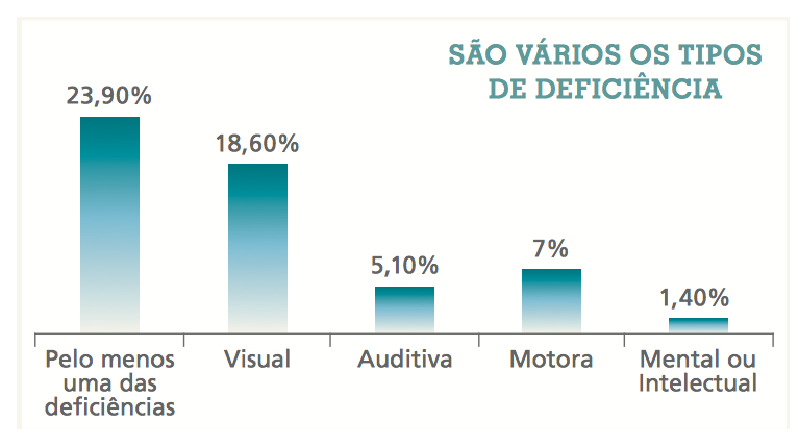
\includegraphics[keepaspectratio=true,scale=0.9]{figuras/censo2010.eps}
	\caption{Proporção sobre a população total residente no Brasil no ano de 2010.}
	\label{censo2010}
\end{figure}

%dificuldades encontradas
Quando se fala sobre a deficiência visual o tema mais discultido é sobre a inclusão social destas pessoas. Segundo \cite{patricia}, para um cidadão, inclusão social significa ter desenvolvimento educacional, estar incluído nas atividades socioeconômicas de seu país, ter acesso às novas tecnologias da informação e conhecimento, para uma ação participativa junto à sua comunidade. Após a promulgação da Constituição de 1988, foi assegurado a igualdade de direitos no trabalho, proteção, integração social e educação social a todos os deficientes. O que esta constituição visa garantir é o reconhecimento social destas pessoas, a proteção e integração, pois elas são igualmente capazes de contribuir com a sociedade e de elaborar sua percepção social. \cite{matos} afirma que: \textit{``A discriminação, o desrespeito à diferença e a persistência de práticas segregativas e excludentes, refletem a falta de princípios éticos, morais e de cidadania.''}. Baseando-se nos pontos levantados, incluir uma pessoa socialmente não se trata apenas de respeito, mas também em oferecer-lhes condições suscetíveis para o desenvolvimento informacional. A busca da igualdade, portanto, contribui no processo de aprendizagem dessas pessoas e não as trata como incapazes. 

Na prática, os cegos ou pessoas com baixa visão não encontram dificuldades apenas ao caminhar na rua ou ao utilizar um transporte público, mas o preconceito, o uso da internet e o acesso a informação também são dificuldades que estas pessoas enfrentam no seu dia a dia. Este fatores influenciam na educação, na alfabetização, no aprendizado e integração social. Crianças brasileiras tem encontrado enormes dificuldade nas salas de aula o que evidencia que apenas a aceitação destas crianças nas escolas não é o suficiente. As escolas não estão preperadas estruturalmente para recebê-las e uma carência de professores capacitados para a formação educacional de crianças com deficiência visual é eminente. O mercado brasileiro de publicações também não oferecem suporte adequado. Este mercado foi avaliado em 2009, após quase 200 anos da criação do braille, e foi considerado incapaz de atender a demanda de livros transcritos o que desfavorece o acesso a informação básica, o processo de educação e o desenvolvimento cultural dos portadores desta deficiência \cite{escolasbrasileiras}. A tecnologia é capaz de oferecer este suporte por meios mais acessíveis proporcionando ao deficiente visual o acesso a informação e consequentemente influenciando positivamente na produtividade e no aprendizado destes \cite{revistaabc}.

Fernando Botelho, aos 17 anos de idade, perdeu completamente a visão e encontrou enormes dificuldades para estudar. Segundo ele, a adaptação foi muito difícil mas ao passar a fazer uso da tecnologia como suporte ao ensino, seu desempenho aumentou consideravelmente tornando-se um dos melhores alunos da universidade. Ele conseguiu concluir a graduação, fez mestrado e hoje viaja o mundo onde sua carreira está sofrendo ascendência cada vez maior. No entanto, Fernando faz parte de um grupo muito pequeno de pessoas que tem acesso a este tipo de tecnologia. Em vista dos 180 milhões de pessoas no mundo que possuem deficiência visual e do alto custo para aquisição desta tecnologia, Fernando está desenvolvendo um programa de computador capaz de auxiliar pessoas com deficiência visual na educação. Segundo ele, é um direito de cada um participar da economia e do meio acadêmico \cite{botelho}. Fundador do F123, projeto que a dois anos desenvolve um software de baixo custo que auxiliará as pessoas com deficiência visual nos seus estudos e profissionalmente, Fernando relata:

\begin{citacao}
O custo alto dos softwares, que já existem no mercado, e a falta de material apropriado para capacitação são os principais fatores para a exclusão de crianças e jovens cegos ou com baixa visão. Os softwares tipicamente usados para a leitura, ou ampliação de tela, custam o equivalente a dois ou três computadores. Este valor elevado impede governos, fundações e organizações de implementarem projetos na escala necessária para obter melhorias significativas, tanto na escolaridade quanto na empregabilidade de jovens com deficiência visual \cite{botelho}.
\end{citacao}

O engenheiro e professor da Faculdade de Tecnologia de Curitiba, Frank Coelho, em uma entrevista cedida para um jornal televisivo de boa audiência, relatou sobre a experiência de vida de Fernando Botelho e o software que está desenvolvendo. Frank disse que: \textit{``Fernando é um gigante que anda no meio de nós mas ele não é um gigante que anda sozinho, ele anda nos ombros de outros gigantes.''}. O Frank estava se referindo ao software livre onde a ideia defendida é que o conhecimento deve ser livre. O trabalho de Fernando foi feito com software livre. Frank defende que esta comunidade pode quebrar com paradigmas e revolucionar a civilização levando o conhecimento as pessoas. Este é o caminho para se conhecer a tecnologia e ajudar as pessoas. Ele também afirma que a tecnologia já está desenvolvida, mas ainda é preciso esforço e disposição para juntar e distribuir.

\subsection{Contraste de Tela}\label{constrastsection}

Após algumas leituras notou-se que cores contrastantes é o conceito mais lembrado quando se fala de contraste de tela para pessoa com baixa visão. As cores contrastantes são cores que, quando usadas próximas umas das outras, produzem uma sensação de choque \cite{griffith}. Na Figura \ref{colors}, as cores mais contrastantes entre si estão diretamente oposta no círculo.

 \begin{figure}[ht]
	\centering
		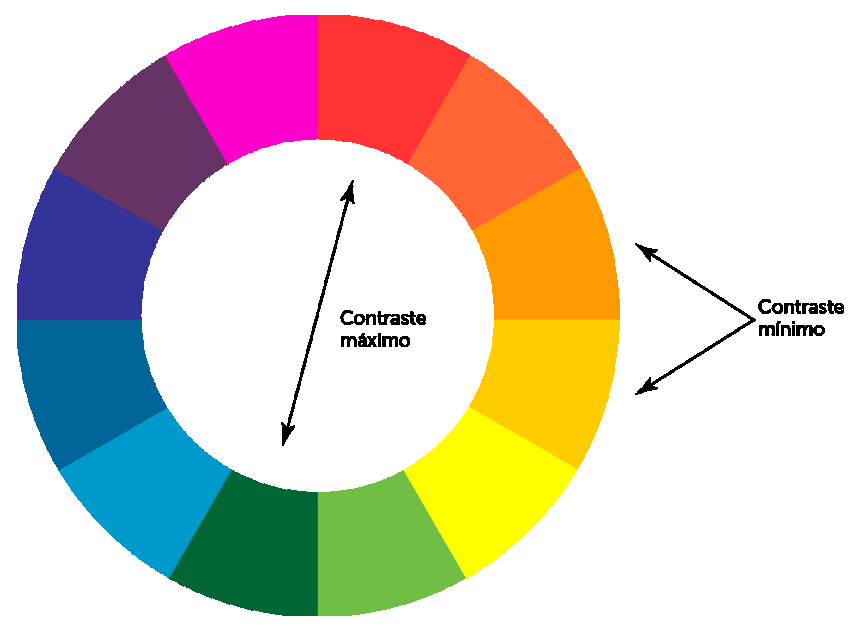
\includegraphics[keepaspectratio=true,scale=0.5]{figuras/contrMatiz.eps}
	\caption{Matriz de contraste de cores (\href{http://ricardoartur.com.br/1001/2011/04/contraste-de-cores/}{fonte}).}
	\label{colors}
\end{figure}

Um artigo escrito por \cite{kulpa} em sua pós-graduação em Design define um modelo de cores na usabilidade das interfaces computacionais para os deficientes de baixa visão. O artigo visa indicar boas práticas na criação ou adequação das interfaces utilizando cores que possibilitem ao deficiente de baixa visão navegar pelo ambiente virtual apenas com sua visão funcional, de forma confortável e satisfatória, sem o auxílio de tecnologias assistivas. Um dos modelos alcançam diversos tipos de diagnósticos de baixa visão e a está representado na Figura \ref{colorscontrast}.

 \begin{figure}[ht]
	\centering
		\includegraphics[keepaspectratio=true,scale=0.5]{figuras/colorscontrast.eps}
	\caption{contrastes que alcançam diversos tipos de diagnósticos de baixa visão.}
	\label{colorscontrast}
\end{figure}

\section{Formatos de Áudio Digital}

O áudio digital refere-se a representação do som (captação por microfone) ou áudio analógico (representado por um vinil ou fita cassete) que é armazenado na forma de um arquivo digital em uma unidade de computador ou outra mídia digital (como \textit{Compact Disc}). O som é contínuo no tempo e para conseguir converter este sinal analógico em sinal de áudio digital, o conversor analógico-digital consiste em ``tirar fotos'' do sinal de áudio em intervalos constantes. Portanto, estas ``fotos'' são uma sequência de amostras que é representado por um sinal de tempo discreto originado da conversão de uma onda de som que, por sua vez, é um sinal contínuo. Assim, definimos \textbf{amostragem} como sendo a redução de um sinal contínuo em um sinal discreto. Em cada uma destas amostras é medido a intensidade do sinal que pode ser representada por 0s e 1s. Ou seja, um áudio digital é a representação binária de um som que é traduzida por um computador ou leitor de CD. Estes são capazes de reproduzir o som original.

Como vimos, o formato de áudio é uma forma de representar digitalmente um som ou um sinal de áudio. Algumas propriedades gerais de representação de som digital são:

\begin{description}
	\item [\textit{bitrate} ou taxa de bits:] que é o número de bits por segundos necessários para representar o sinal. O \textit{bitrate} descreve, então, a velocidade com que o som é reproduzido (por exemplo, 320 000 bits por segundos ou 320 Kbps);
	\item [\textit{number of channels} ou número de canais:] usa-se, tradicionalmente, um canal (som mono) ou dois canais (som estéreo); 
	\item [\textit{sampling frequency} ou frequência de amostragem:] define o número de amostras que são coletadas em um tempo pré determinado e a unidade de medição é dada em \textit{Hertz}. As amostras são medidas em intervalos fixos.
\end{description}

Com o avanço e popularidade da digitalização do som, o áudio digital tem sido largamente usado. Um dos principais motivos é a facilidade no uso deste tipo de arquivo, pois trabalhar com um sinal digital é muito mais simples se comparado ao sinal analógico. Os formatos são geralmente conhecidos por sua extensão e não pelo seu nome. Existem diversos formatos de áudio digital, mas primeiro vamos falar sobre o PCM.

\subsection{Formatos não comprimidos}

%citar formatos
Os formatos não comprimidos possuem qualidade máxima pois não há alteração dos bits do ficheiro de áudio. Isto faz dos formatos não comprimidos útil para aplicações profissionais. O áudio digital é armazenado sem realizar a compressão dos dados e, portanto, demandam grande espaço em memória.

%falar dos formatos dos arquivos de áudio
\subsection{PCM}

Com seu surgimento na década de 30 por Alec Reeves, o PCM (\textit{do inglês, Pulse Code Modulation - Modulação por Código de Pulso}) é a forma mais antiga de digitalização do som e o mais utilizado devido à reprodução fiel do som, que é armazenado. Isso significa que os dados foram levados diretamente a partir da entrada, digitalizada e armazenada sem transformação. Não havia compressão de dados na época pois o poder de computação era escasso \cite{pcm}.


Como explanado no início desta seção, a digitalização não é contínua, ou seja, não é constante como o som. Por possuir valores discretos (descontínuos), a digitalização sonora envolve dois parâmetros básicos: a frequência de amostragem e a profundidade de bit. A \textbf{profundidade de bit} (\textit{bit depth}) trata da quantidade de bits de computador que são usados para representar cada amostra. Uma representação com um bit recebe apenas dois valores (0 e 1). Se tenho uma representação com 4 bits é possível receber 16 valores diferentes onde a amplitude de cada amostra é um dos 16 valores possíveis \cite{pcm}. A taxa de amostragem e a amplitude influenciam diretamente na qualidade do áudio. Sony e Philips desenvolveram a tecnologia PCM e criaram o \textit{Compact Disc}. O CD possui 44100 amostras por segundo e uma amplitude de 16 bits o que torna a qualidade alta.


\subsection{Formato WAV}

O formato \textit{Waveform Audio Format} ou WAVE (os ficheiros deste formato utilizam a extensão *.wav) possui o seu áudio codificado em PCM. Criado pela Microsoft, este formato de áudio digital é nativo do sistema operativo Windows e é compatível com quase todos os tocadores atuais. Um ponto negativo é o tamanho de seu arquivo que chega a possuir uma média de 10 MB por minuto \cite{serraaudio}.

O WAV é derivado do padrão IFF criado pela \textit{Eletronic Arts Interchange File Format} onde seu conteúdo é divido em blocos denominados \textit{chunks}. Existem diversos tipos de \textit{chunks} em um arquivo WAV, mas apenas dois são obrigatórios (além do chunk \textit{header} que especifica o formato do áudio).

\begin{description}
	\item [\textit{fmt chunk}]: define algumas informações sobre o formato do arquivo tais como número de canais, sua taxa de amostragem e o tamanho de seus \textit{samples};
	\item [data \textit{chunk}]: responsável por armazenar a sequência de \textit{samples}.
\end{description}

A Figura \ref{wave} ilustra o que foi explicado sobre a estrutura geral de um formato WAVE.

 \begin{figure}[ht]
	\centering
		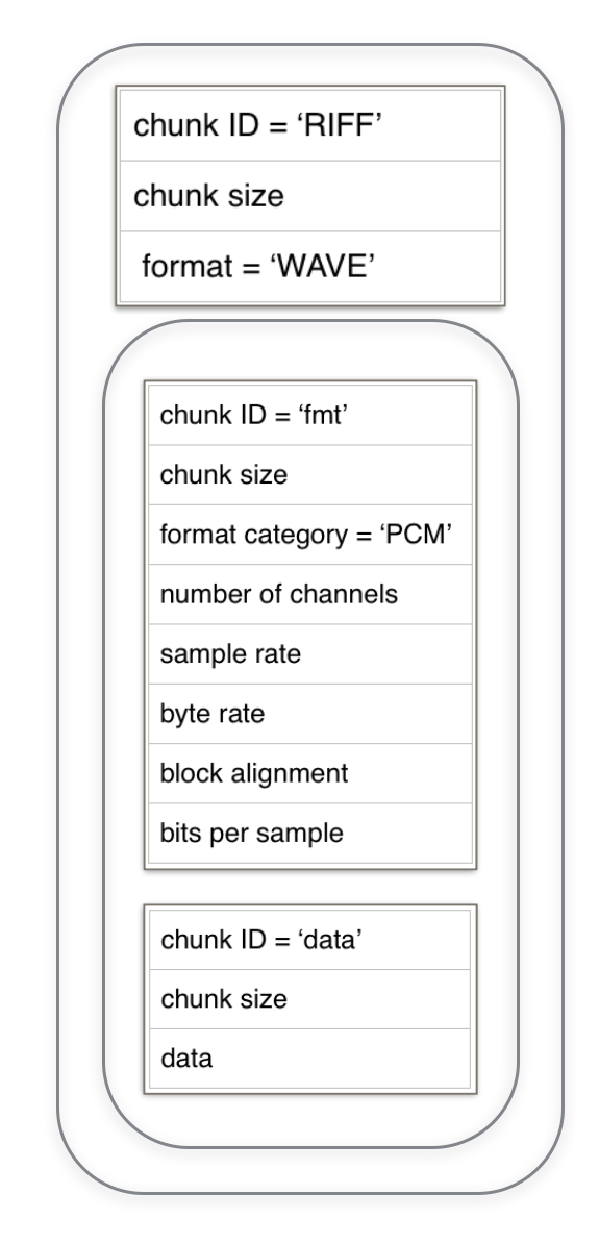
\includegraphics[keepaspectratio=true,scale=0.5]{figuras/wave.eps}
	\caption{Diagrama Geral do formato WAVE.}
	\label{wave}
\end{figure}

\subsection{Formato AIFF}

O formato \textit{Audio Interchange File Format} (a extensão destes ficheiros pode ser *.aiff ou *.aif) é bastante similar ao WAV. Foi criado pela Apple e portanto é bastante popular e nativo em seu sistema operacional. O AIFF possui áudio em formato PCM porém não é tão difundido quanto o formato WAV. Como o nome sugere, o AIFF também usa o método IFF para armazenar seus dados e também possui dois \textit{chunks} obrigatórios: o \textit{common chunk} e o \textit{sound data chunk} \cite{muratnkonar}. A Figura \ref{aiff} ilustra, de forma geral, como um formato AIFF de áudio é estruturado.

 \begin{figure}[ht]
	\centering
		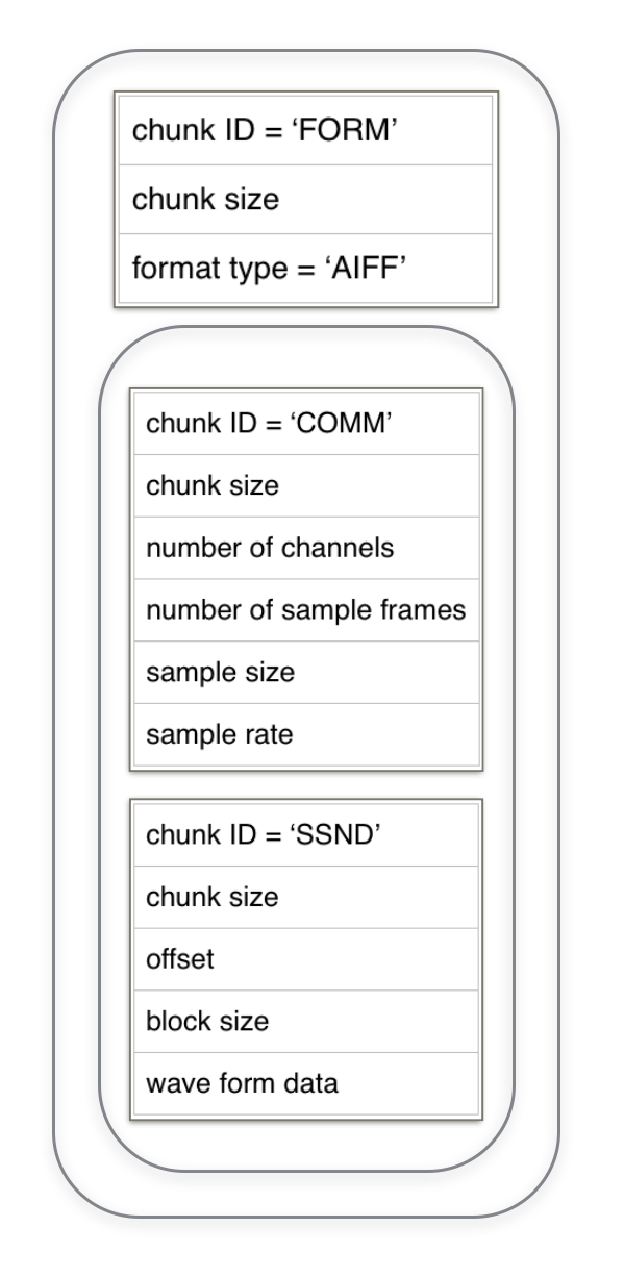
\includegraphics[keepaspectratio=true,scale=0.5]{figuras/aiff.eps}
	\caption{Diagrama Geral do formato AIFF.}
	\label{aiff}
\end{figure}

\begin{description}
	\item [\textit{common chunk}:] define algumas informações fundamentais do formato do como visto na Figura \ref{aiff};
	\item [sound data \textit{chunk}:] responsável por armazenar a sequência de \textit{sample frames}.
\end{description}

\subsection{Formatos comprimidos}

Os formatos comprimidos possuem qualidade inferior aos formatos não comprimidos. Todavia, dependendo da compressão feita, mesmo com um pouco da perda da qualidade, a alteração é imperceptível. Por conta da compressão é possível obter um ficheiro de áudio com qualidade boa e com o espaço ocupado em memória reduzido.

\subsection{Formato MP3}

O MPEG-1 Layer 3 (popularmente conhecido com MP3) é a primeira versão do codec MPEG que é utilizada, atualmente, para codificar áudio. O MPEG, do inglês \textit{Moving Picture Experts Group} é um padrão que define técnicas de compressão de áudio e vídeo. A Camadas (\textit{Layers}) diferem-se em termos de qualidade, sendo as primeiras dotadas de qualidades superiores e consequentemente voltadas para uso profissional de áudio como em estúdios de gravação. A Camada 3 foi adotada para o consumidor final por ser capaz de gerar arquivos com boa taxa de compressão e áudio de boa qualidade. O MP3 é construído a partir de pequenas partes chamadas \textit{frames}. Cada frame, por sua vez, é composto por um \textit{header} e um bloco de dados \cite{mpgedit}. A Figura \ref{mp3} melhor define esta estrutura.

 \begin{figure}[ht]
	\centering
		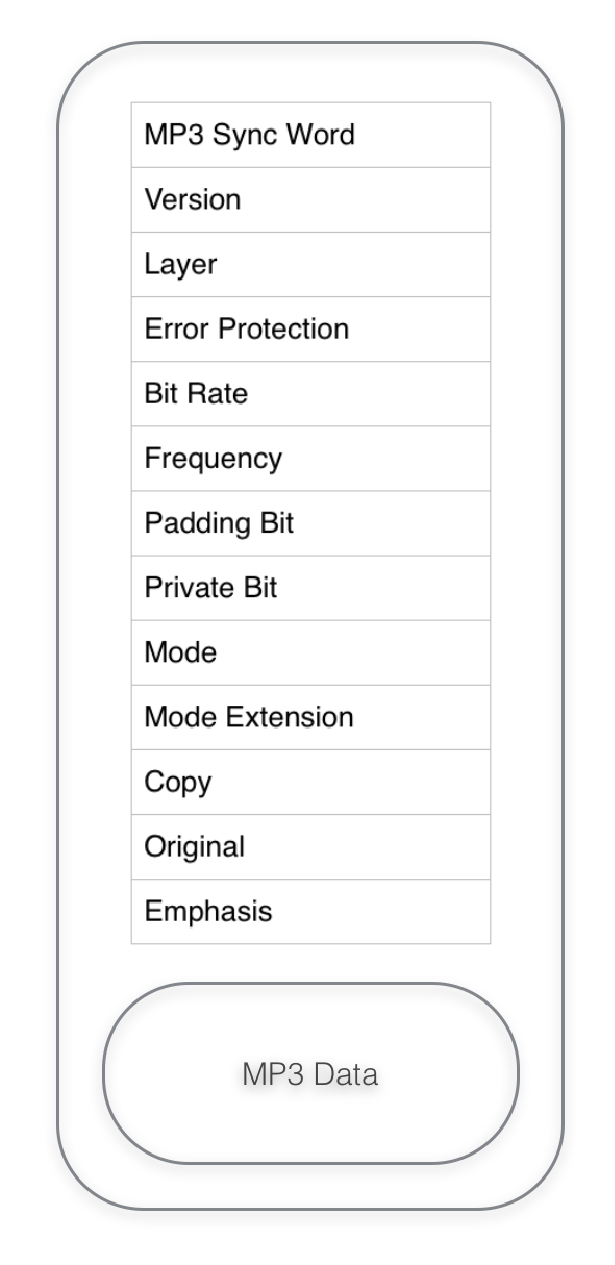
\includegraphics[keepaspectratio=true,scale=0.5]{figuras/mp3.eps}
	\caption{Diagrama Geral representando um \textit{frame} do formato MP3.}
	\label{mp3}
\end{figure}

O MP3 se popularizou através de um software criado por Shawn Fanning chamado Napster. Apesar da rede Napster ter tido uma vida curta (cerca de 2 anos), o programa fez bastante sucesso sendo o percursor do compartilhamento de arquivos de áudio em formato MP3. Por conta da dificuldade em encontrar áudios em formato MP3, Fanning criou o programa para compartilhar estes ficheiros de áudio entre amigos. Usando da tecnologia P2P (\textit{peer to peer}) e pela popularidade entre os amigos, o programa foi copiado para diversas outras pessoas alcançando pessoas ao redor do mundo \cite{mp3oquee}. Dentre os formatos de áudio, o MP3 é o mais popular. O grande problema dele é sua patente.


%\subsection{Formato Ogg Vorbis}

%Será visto na seção \ref{cap3.4}.

%\section{Compressão de Dados}

%A compressão de dados é uma técnica utilizada para que um arquivo de dados ocupe um menor espaço em memória física, reduzindo assim a dimensão física de blocos de informação. Esta compressão se dá pela diminuição da quantidade de bits ou até mesmo de bytes que representam um dado. Todos os dados computacionais como texto, imagens, músicas e vídeos são compostos por uma série de bits, sendo o bit uma unidade atômica de armazenamento, que podem ser representados por bytes que consistitui-se do conjunto de oito bits \cite{tenenbaumdados}. Um dado pode ser comprimido sem nenhuma perda, por meio de algoritmos de compressão, retirando-se informações redundantes. É percepitível o motivo de compressão para economizar espaço em dispositivos de armazenamento. No entanto, os dados também são comprimidos para um ganho de desempenho em transmissões. Sayood, atual professor da Universidade de Nebraska-Lincoln, escreveu:

%\begin{citacao}
%Compressão, redução da taxa de bits e redução de dados têm basicamente o mesmo significado, ou seja, quer se obter a mesma informação porém utilizando menor quantidade de dados. Há vários motivos para que a compressão se torne popular. Podemos citar a diminuição da quantidade de memória necessária para o armazenamento (hardware menor), o menor custo devido a uma menor largura de banda requerida para a transmissão da mesma quantidade de dados e a facilidade nas transmissões em tempo real \cite{sayood}.
%\end{citacao}

%Além da redundância, um outro fator que pode ser levado em consideração é a irrelevância da informação. Diferente do caso anterior, a irrelevância necessariamente ocasionará em perda de informação. Existem diversos métodos de compressão de dados. Apesar da existência de outros, a forma mais conhecida de se classificar métodos de compressão de dados é pela ocorrência ou não de perda de dados durante o processo. Apesar do computador manipular todas as informações por bits, o método de compressão depende intrinsecamente do tipo de dado a ser comprimido \cite{compressaoadaptativa}.

%\subsection{Compressão sem perda de dados}

%A compressão sem perda de dados tira partido da redundância. Este tipo de compressão deve ser capaz de reconstruir, após a descompressão por meio de algoritmos de compressão, a informação original sem nenhuma perda de informação. Podemos citar como exemplo os ficheiros executáveis. Este tipo de dado deve ser recuperado sendo necessário a conservação da sua integridade para que funcione corretamente. Ou seja, este método de compressão é reversível sendo possível reconstruir o dado mantendo sua integridade e a mesma qualidade.

%\subsection{Compressão com perda de dados}

%A compressão com perda de dados tira partido da redundância e da irrelevância. Este tipo de compressão não é capaz de reconstruir, após a descompressão por meio de algoritmos de compressão, a informação original. Porém, é suficientemente parecida para que seja útil de alguma forma ou sua diferença imperceptível. Este tipo de método de compressão é comumente utilizado para arquivos de áudio e vídeo. Os dados multimídia podem tolerar um certo nível de degradação sem que a percepção humana, como olho e tímpano, distingam uma degradação significativa. Para exemplificar, as frequencias de som em que a audição humana não é capaz de captar é eliminado por este tipo de compressão. O arquivo passa a ter uma qualidade reduzida porém uma alta taxa de compressão.

%\subsection{Compressão de áudio}

%Como explanado nos tópicos anteriores, é de suma importância comprimir dados e com o áudio não é diferente. Com a compressão de áudio há uma melhoria no fluxo de dados minimizando os esforços computacionais nas tarefas de transmissão de dados e armazenamento. Isto facilita a execução de serviços de comunicação em tempo real e gera um aumento de desempenho das aplicações \cite{compressaoaudio}.

%Geralmente, a compressão de áudio é feita com perda de dados. Numa música, pode ocorrer uma redundância de informação a partir do momento em que longos períodos de amostras de som possuem o mesmo valor. Para eliminar a repetição desnecessária de informação, por exemplo, os trechos das amostras de som de mesmo valor poderiam ser substituídos por um pequeno código dizendo que a mesma frequência deve ser repetida um número determinado de vezes. Outro tipo de redundância é os momentos de silêncio num sinal de áudio. Até certo ponto é possível comprimir o som sem nenhuma perda de qualidade, mas, para que possamos comprimir ainda mais um ficheiro de áudio, podemos abrir mão de uma pouco da qualidade de áudio para geração de arquivos ainda menores. No entanto, além das técnicas habituais de compressão, aproveita-se o conhecimento das imperfeições ou limitações na audição. Usando da irrelevância da informação e com prévio conhecimento das características da audição humana, podemos eliminar certas informações sem afetar o que ouvimos. Segundo \cite{compressaoaudio} ``Porém, biologicamente, podemos afirmar que o ouvido humano somente responde a certas faixas de frequência''. Ou seja, existe uma pequena perda da qualidade do áudio mas são inaudíveis para o ser humano. Assim podemos afirmar que a qualidade é mantida, pois ``Por definição, o som de qualidade de um codificador só pode ser determinado pelo ouvido humano.'' \cite{compressaoaudio}.

%\subsection{Porque comprimir os dados?}

%Com o avanço tecnológico, a manipulação de dados tem exigido cada vez mais poder de processamento e capacidade de armazenamento. Com o crescente desenvolvimento das aplicações que manipulam dados multimídia para entretenimento dos usuários, há um aumento da quantidade de informação que é passada através das redes. Estes tipos de dados, tais como som, imagem e vídeo, ocupam grande espaço em disco o que dificulta o uso das redes para compartilhamento destes dados. Considere um áudio codificado a uma taxa de amostragem de 44.1Hz, 16 bits por amostra e estéreo. Este áudio possui qualidade de CD. Vamos definir a largura de banda necessária para a transmissão deste áudio. Para tal, basta multiplicar os valores destas três informações \cite{forouzan}. Se multiplicarmos a frequência de amostragem pelos bits de cada amostra, nós teremos o número de bits por segundo. No entanto, ainda devemos multiplicar este valor por dois, pois o áudio está no modo estéreo. Este modo utiliza dois canais de som sincronizados no tempo. Assim, teremos o valor de 1.411.200 bits por segundo. Isto significa que para transmitir tal arquivo por uma rede, é necessária uma largura de banda de 1,41 Mbits/s. Para sabermos qual o espaço utilizado por este áudio para armazená-lo em um computador precisamos, primeiramente, saber qual a sua duração. Se dissermos que o áudio possui 180 segundos de duração e temos 1.411.200 bits por segundo, estimasse que este áudio possui 254.016.000 bits o que é equivalente a um pouco mais de 30MB \cite{forouzan}. Este dois exemplos dão uma ideia da importância da compressão de áudio.


%Além dos fatores espaço de armazenamento e compartilhamento de dados através das redes, estes dados também tem grande influência no que tange o desempenho das aplicações. O poder de processamento tem crescido mais rapidamente do que as capacidades de armazenamento e desempenho no uso da memória. Em 1965, Gordon Earl Moore previu que o poder de processamento dos computadores dobrariam a cada 18 meses. Essa observação ficou conhecida como Lei de Moore. \cite{moore} e \cite{tanenbaumorganizacao}. A Figura \ref{graphicmoore} informa dados pontuais onde é possível observar a evolução da quantidade de componentes por chip para os microprocessadores da Intel entre 1970 e 2005.

 %\begin{figure}[ht]
%	\centering
%		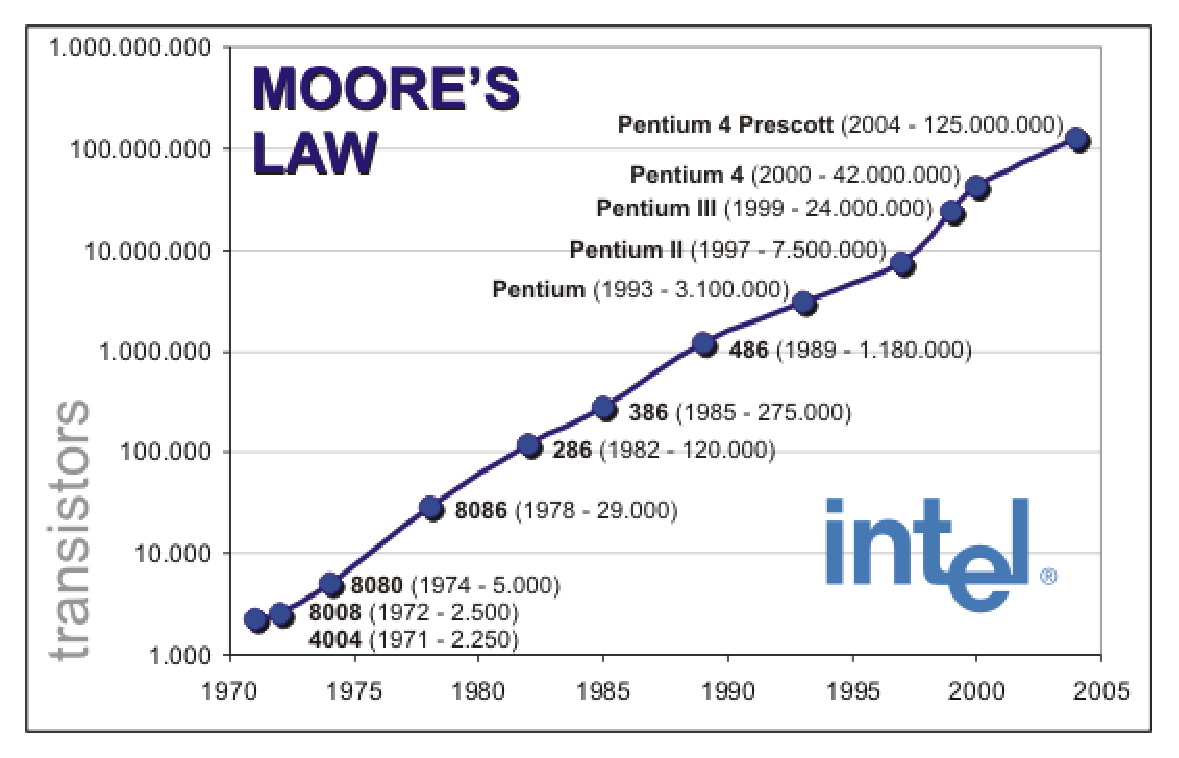
\includegraphics[keepaspectratio=true,scale=0.5]{figuras/graphicmoore.eps}
%	\caption{Lei de Moore em ação para microprocessadores Intel \cite{phonearena}}
%	\label{graphicmoore}
%\end{figure}

%Apesar do poder de processamento ter crescido exponencialmente, ele não é o único fator que influencia no desempenho de uma aplicação. Um computador, basicamente, trabalha com dados e para manipulá-los o processador faz requisições a memória, seja para gravar algum dado em disco ou obter dele. Estas requisições feitas ao disco leva um tempo considerado altíssimo e isto reduz o desempenho de uma aplicação apenas pelo acesso feito a memória \cite{tanenbaumorganizacao}. Ou seja, o processador acaba ficando ocioso esperando as instruções ou operandos que estão sendo buscados na memória durante a execução de instruções. A capacidade de armazenmento também está ligada a taxa de transferência de dados. Quanto maior a capacidade, maior será o tempo de acesso. Outro fator limitante para o uso de memórias com capacidades cada vez maiores é o seu custo. Para que um sistema seja comercialmente viável, o custo da memória deve ser compatível com os demais componentes \cite{tanenbaumorganizacao}. 

%De acordo com \cite{cloud}, entre os anos 2012 e 2017 os recursos por mais processamento, armazenamento de dados e comunicações poderá triplicar. Este crescimento de dados foi atribuído, representando 50\% do aumento, ao crescimento de streaming de vídeo e áudio. Em horários de pico, 50\% do tráfego de Internet são dados trafegados do Netflix e Youtube \cite{cloud}.

%A compressão dos dados é importante para a redução de dados como áudio, imagens e vídeos em situações como transmissão de dados ou armazenamento, pois é ideal a diminuição do tempo de latência. Desta forma, o custo para transmissão dos arquivos na rede ou para a taxa de transfência para a/da memória será menor. O problema de economia de memória, apesar das memórias terem se tornado maiores se comparadas em épocas passadas, ele ainda permanece nos dias de hoje. Como vimos, os custos para acessar os dados em memória ainda é alto, ocasionando na perda de desempenho \cite{tanenbaumorganizacao}. A compressão de dados é um dos fatores que mais contribuiu para o grande cescimento das tecnologias da informação e da comunicação. Sem compressão, a maioria dos produtos tecnológicos de consumo e entretenimento nunca teria chegado a existir como, por exemplo, as câmeras fotográficas digitais, DVDs, leitores de MP3, o Youtube e o streaming de vídeo, as redes sem fio e a televisão digital. De fato, as tecnologias de compressão multimídia permitem representar a informação de uma forma mais eficiente, reduzindo os grandes volumes de espaço de armazenamento que ocupa e, portanto, a largura de banda que consome para se transmitir nas redes e na Internet \cite{compressaomultimidia}. 


%\section{Formato Ogg Vorbis}\label{cap3.4}

%Conhecido por seu método de compressão de áudio digital e por ser livre de patentes, o codec de áudio Ogg Vorbis surgiu a partir da junção de dois projetos desenvolvidos pela Xiph.org. O projeto Ogg é um formato recipiente que armazena qualquer tipo de conteúdo multimédia digital. O contêiner multimédia (assim chamado pela Xiph.org) pode conter informações de textos, áudio e vídeo e tem sido usado para encapsular dados comprimidos de outros codecs \cite{ogg}. O projeto Vorbis, por outro lado, é um \textit{codec} responsável pela compressão e descompressão de áudio e foi projetado para ser contido em um ficheiro Ogg \cite{vorbis}. O \textit{codec} é o termo utilizado para algoritmos que realizam codificação e decodificação de um fluxo de dados digital. Este dois projetos podem ser usados separadamente ou em conjunto com outros formatos e \textit{codecs}.

%O Ogg Vorbis visa substituir completamente todos os formatos patenteados e proprietários. Ele foi criado para concorrer, principalmente, com os codecs MP3 e o AAC. O formato foi iniciado logo após a organização Fraunhofer Gesellschaft (responsável por projetar o algortimo de compressão do formato MP3 patenteado pela Fraunhofer IIS) anunciar os seus planos de cobrar licenças de uso para o formato MP3.

%Apesar de ser um formato não proprietário, o Ogg Vorbis consegue melhores taxas de compressão e qualidade de áudio superior que o MP3. Uma desvantagem do Ogg Vorbis é sua compressão ser quase duas vezes mais lenta, mas isso pode ser resolvido no futuro. O Ogg pode não ser tão popular quanto o MP3, todavia, tem sido cada vez mais conhecido e melhorado. No ramo de jogos, o Ogg tem sido consideravelmente usado.


\subsection{Formato Ogg}

O resultado de um encapsulamento Ogg é chamado de \textbf{\textit{Pyshical Ogg Bitstream}}. O Ogg encapsula dados comprimidos criado por codecs. Os dados comprimidos são fluxos de bits de mídia que é chamado de \textbf{\textit{logical bitstreams}} e pode ser representados por um fluxo simples de áudio Vorbis, múltiplos fluxos de áudio ou fluxos de áudio e vídeo multiplexados. Um \textit{logical bitstream} é estruturado, ou seja, ele é dividido em uma sequência de \textbf{\textit{packets}}. Os pacotes são criados pelo codificador de \textit{logical bitstream} e estes pacotes apenas tem representação para o codificador: ``Please note that the term packet is not used in this document to signify entities for transport over a network'' \cite{ogg}.

O Ogg oferece suporte para o transporte do fluxo de bits lógicos como enquadramento e intercalação para diferentes fluxos. O formato também é capaz de detectar corrupção e recuperar-se após algum erro de análise. Marcos de posição é suportado e, dessa forma, torna-se possível o acesso aleatório direto de posições arbitrárias na \textit{bistream}. Outra forte característica é a capacidade de streaming, onde não é necessário a construção completa do \textit{bitstream} para a transmissão do mesmo. Outros suporte, e não menos importante, é a pequena sobrecarga referente a largura de banda do bitstream.

O \textit{Pyshical Ogg Bitstream} consiste de vários \textit{logical bitstreams} intercalados em \textbf{\textit{Pages}}. O \textit{logical bitstream}  são indentificados por um número de série único no cabeçalho de cada \textit{page}. As \textit{pages} são intercaladas simultaneamente e não precisam seguir uma ordem regular, mas precisam ser consecutivos dentro de um \textit{logical bitstream}. A desmultiplexação Ogg é capaz de reconstruir o \textit{logical bitstream} original. Cada \textit{page} contém apenas um tipo de dado, uma vez que pertence a um único \textit{logical bitstream}. As \textit{pages} possuem tamanhos variáveis e tem um cabeçalho contendo encapsulamento e recuperação de erros de informação. Cada \textit{logical bitstream} em um \textit{physical Ogg bitstream} começa com uma páginal inicial especial \textbf{bos} (\textit{beginning of stream}) e termina com uma página especial \textbf{eos} (\textit{end of stream}) \cite{ogg}.

Uma página bos contém informações para identificar o tipo de codec e pode conter informações para configurar o processo de decodificação. Ela também deve conter informações sobre os meios de comunicação codificada. Para exemplificar, uma página bos, para um áudio, deve conter a taxa de amostragem e o número de canais. Por convenção, os primeiros bytes de uma página bos contém informações necessárias para identificação do \textit{codec}. O Ogg também permite mas não obriga pacotes de cabeçalhos (\textit{header packets}) secundários após a página bos para o \textit{logical bitstream} e estes devem preceder quaisquer pacotes de dados (\textit{data packtes}) em qualquer \textit{logical bitstream}. Este pacotes de cabeçalhos são enquadrados em um número integral de páginas e estas, por sua vez, não contém quaisquer pacotes de dados. Portanto, conclui-se que um \textit{physcial Ogg bitstream} começa com as páginas de todos os \textit{logical bitstreams} contendo um pacote de cabeçalho inicial por página, seguido por pacotes de cabeçalhos subsidiários  de todos os fluxos e, por fim, seguido pos páginas contendo pacotes de dados \cite{ogg}.

 A especificação de encapsulação de um ou mais \textit{logical bitstreams} é chamado de  \textbf{\textit{media mapping}}  ou mapeamento de mídia. A \cite{ogg} exemplifica um mapeamento de mídia citando o ``Ogg Vorbis'', que usa a estrutura Ogg Vorbis para encapsular os dados de áudio codificados para armazenamento baseado em arquivo e transmissão baseada em fluxo. O Ogg Vorbis fornece o nome do \textit{codec} e algumas informações referentes ao áudio codificado. Ele também possui duas páginas adicionais de cabeçalho. A página bos do Ogg Vorbis começa com o byte 0x01, seguido por ``Vorbis'' totalizando 7 bytes de identificador. O \textit{codec} Vorbis será visto na seção 2.4.2.

\subsubsection{Mutiplexagem}

 O formato possui dois tipos de multiplexagem: \textit{grouping} (agrupamento) e \textit{chaining} (encadeamento). No \textbf{\textit{grouping}} a multiplexação é simultânea onde vários \textit{logical bitstreams} são intercalados em um mesmo \textit{physical bitstream} como, por exemplo, a intercalação de um fluxo de vídeo com diversas faixas de áudio. É importante ressaltar que na multiplexagem \textit{gouping} todas as páginas bos de todos os \textit{logical bitstreams} devem aparecer juntas no início do \textit{physical Ogg bitstream}. Por outro lado, as páginas eos não precisam estar lado a lado. A multiplexagem \textbf{\textit{chaining}}, por sua vez, foi definido para proporcionar um mecanismo simples de concatenação do \textit{physical Ogg Vorbis} onde os \textit{logical bitstreams} completos são concatenados. O \textit{chaining} são frequentemente usados em aplicações de transmissão. Não há sobreposição dos \textit{bitstreams} pois a página eos de um dado \textit{logical bitstream} é imediatamente seguido pela página do próximo bos \cite{ogg}. Os dois tipos de multiplexagem podem ser usados em conjunto. A Figura \ref{multiplexogg} é um diagrama que representa os dois tipos de multiplexagem.

 \begin{figure}[ht]
	\centering
		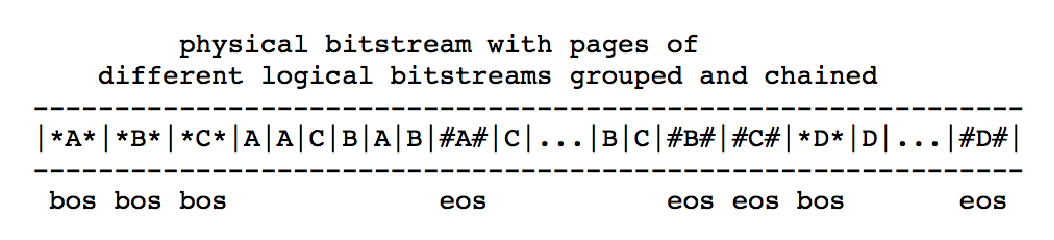
\includegraphics[keepaspectratio=true,scale=0.7]{figuras/multiplexogg.eps}
	\caption{Diagrama exemplificando as multiplexagens \cite{ogg}}
	\label{multiplexogg}
\end{figure}

O Ogg não sabe nada sobre os dados do \textit{codec} que ele encapsula e é, portanto, independente de qualquer codec de mídia. A exceção para aquilo que o Ogg conhece é que cada \textit{logical bitstream} pertence a um \textit{codec} diferente, os dados do \textit{codec} vem em ordem e possuem marcadores de posição (são \textit{granule positions} que serão abordados mais a frente). O recipiente Ogg não possui conceito de tempo. No entanto, o Ogg sabe sobre o aumento sequencial dos marcadores de posição. Isto faz do Ogg uma estrutura genérica mas que realiza o encapsulamento de fluxos de bits de tempo contínuo.

O processo de multiplexação ocorre no nível de página. Porém, os \textit{codecs} fornecem fluxos de bits que são entregues ao Ogg em pacotes de tamanho arbitrário e não limitado. As páginas, em contra partida, possuem tamanho máximo de 64 Kbytes. Desta forma, os pacotes, na maiora das vezes, precisam ser distribuídos ao longo de várias páginas. Para realizar essa distribuição e facilitar o processo, o Ogg quebra um pacote em \textbf{segmentos} de 255 bytes sendo o último segmento mais curto. Os segmentos são apenas uma construção lógica e não tem um cabeçalho para si. Uma \textit{flag} no cabeçalho da página informa se uma página contém informações de um pacote de continuação da página anterior \cite{ogg}. Para um melhor entendimento, a Figura \ref{segments} é um diagrama que exemplifica a relação entre páginas, pacotes e seguimentos.

\begin{figure}[ht]
	\centering
		\includegraphics[keepaspectratio=true,scale=0.6]{figuras/segments.eps}
	\caption{Representação da disposição dos segmentos \cite{ogg}}
	\label{segments}
\end{figure}

Um cabeçalho de página contém todas as informações necessárias para a desmultiplexação dos fluxos de bits lógicos e para executar a recuperação de erros básicos e marcos para a procura. Cada página é uma entidade auto-suficiente de modo que o mecanismo de página de decodificação pode reconhecer, verificar e lidar com páginas simples em um momento sem ser necessário todo o fluxo de bits. A Figura \ref{pageheader} define o formato para um cabeçalho de página.

\begin{figure}[ht]
	\centering
		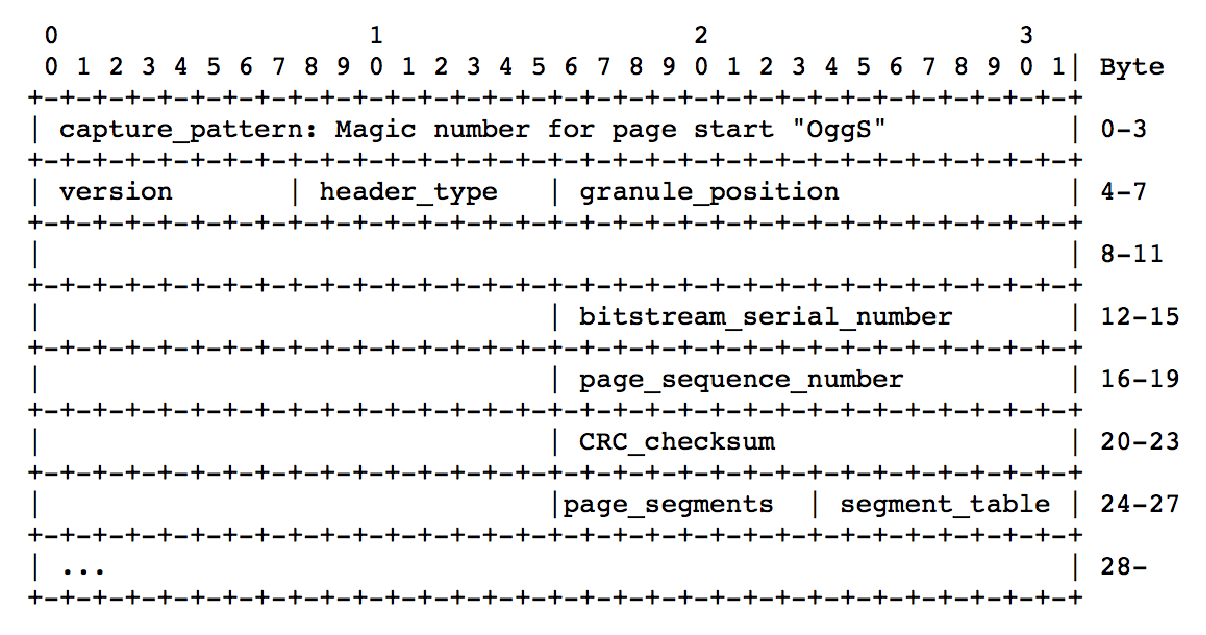
\includegraphics[keepaspectratio=true,scale=0.6]{figuras/pageheader.eps}
	\caption{Formato de cabeçalho de uma página \cite{ogg}}
	\label{pageheader}
\end{figure}

Segundo \cite{ogg}, os campos da estrutura da Figura \ref{pageheader} possuem os seguintes significados:

\begin{itemize}
	\item{\textbf{\textit{capture\_pattern}}:} cada página começa com uma \textit{string} de quatro bytes ``OggS''. As letras ``O'' e ``S'' devem ser maiúsculas e suas representações na tabela ASCII dadas em hexadecimal são 0x4f e 0x53, respectivamente. A letra minúscula ``g'' é representada por 0x67. Se a sincronização for perdida, este campo ajuda o decodificador na recuperação da sincronização;
	\item{\textbf{\textit{version}}:} especifica a versão do arquivo Ogg e possui 1 byte para sua representação;
	\item{\textbf{\textit{header\_type}}:} Este campo possui apenas um byte. No entanto, os bits identificam o tipo específico de cada página:
	\subitem{\underline{bit 0x01}}: se este bit for igual a 1, significa dizer que a página contém dados de um pacote de continuação da página anterior. Caso seja 0, a página está iniciando um novo pacote;
	\subitem{\underline{bit 0x02}}: se o bit estiver setado como um, então é uma página bos. Se o bit for 0, significa que não é uma primeira página;
	\subitem{\underline{bit 0x04}}: se o bit estiver setado como um, então é uma página eos. Se o bit for 0, significa que não é a última página.
	\item{\textbf{\textit{granule\_position}}:} Os 8 bytes (ou 64 bits) que representa este campo, contém informações referente a posição. O Ogg não contém informações de tempo, porém o tempo é mapeado referente a posição de um dado digital em uma \textit{stream}. O significado real deste campo em relação ao tempo depende de cada \textit{codec};
	\item{\textbf{\textit{serial\_number}}:} o \textit{logical bitstream} é identificado com um único número de série neste campo de 4 bytes;
	\item{\textbf{\textit{sequence\_number}}:} se o campo anterior identifica um \textit{logical bitstream} este campo contém o número de sequência da página que é incremetnado separadamente. O campo também possui 4 bytes e através dele o decodificador consegue identificar a perda de página;
	\item{\textbf{\textit{CRC\_checksum}}:} contém CRC checksum de 32 bits cujo polinômio gerador é 0x04c11db7;
	\item{\textbf{\textit{page\_segment}}:} este campo possui um 1 byte de tamanho e fornece o número de entradas de segmentos codificados na tabela de segmentos;
	\item{\textbf{\textit{segment\_table}}:} contém informações de \textit{lacing values} de todos os seguimentos contido na página. Cada byte deste campo contém um valor de laço e, portanto, o número de bytes deste campo é igual a quantidade de segmentos existentes na página. 
\end{itemize}

\subsection{\textit{Codec} Vorbis}

% O Vorbis é um \textit{codec} de áudio usado para comprimir sinal de áudio e esta seção fornece uma descrição em alto nível sobre o método de codificação e decodificação bem como a forma com que o projeto Vorbis foi estruturado.

O \textit{codec} Vorbis codifica blocos PCM de curta duração em pacotes de bits de dados comprimidos. Ele não fornece nenhum tipo próprio de enquadramento, sincronização ou proteção contra erros. Para isso, Vorbis utiliza do formato de fluxos de dados do Ogg para disponibilizar sincronização, recaptura de sincronização após erros, marcadores durante a procura e informação suficiente para separar corretamente os pacotes de dados codificados para obter o pacote original. Segundo sua especificação \cite{vorbis}, Vorbis é apenas um método de aceitação de entrada de áudio, dividindo este áudio em \textit{frames} (quadros) individuais comprimidos que são pacotes não formatados. Basicamente, o decodificador aceita estes pacotes em sequência, decodifica-os e os sintetiza no fluxo do áudio original.

Para obter arquivos cada vez menores e com uma qualidade constante, o Vorbis utiliza uma codificação de débito binário variável. O \textbf{VBR} (\textit{Variable Bit Rate}) é um algoritmo que define qual a melhor taxa de bit para cada frame da música variando, assim, a quantidade de transferência de bits por segundo mas mantendo a qualidade constante \cite{vbr}. Ou seja, O Vorbis é um formato de taxa variável e seus pacotes não possuem tamanho fixo e depende do parâmetro de qualidade. O nível de qualidade varia de 0 a 10 com mudanças feitas de 1 em 1. A qualidade 0 corresponde a 64 Kbps, 5 por volta de 160 Kbps e 10 cerca de 400 Kbps. O nível cinco de qualidade já é suficiente para se aproximar de uma qualidade de áudio de CD. Portanto, ao usar o VBR, o Vorbis consegue atingir qualidade de som semelhante ao original e com melhor compressão. A taxa de bits varia de 16 Kbps a 500 Kbps por canal. O número de canais de áudio independentes suportados podem chegar a 255 \cite{vorbis}. No entanto, o nível 3 é mais utilizado por conseguir, a partir de 110 Kbps, gerar ficheiros de áudio menores e qualidade superior a ficheiros MP3 com 128 Kbps.

%Os codebooks contém  os códigos de Huffman e quantizações vetoriais

\subsubsection{Algortimo de compressão}

Os métodos usados para a compressão de áudio geralemente pertencem a duas categorias: métodos que trabalham no domínio do tempo e métodos que trabalham no domínio da frequência. Todos os formatos conhecidos que trabalham no domínio da frequência usa a transformada discreta do cosseno modificada. O \textbf{MDCT} (\textit{Modified Discrete Cosine Transform}) realiza a tranformação para o domínio da frequência a partir do domínio do tempo. O \textbf{\textit{window shape}} que contém amostras PCM com duas variações de comprimentos especificados em 2048 ou 512 amostras. O Vorbis usa o MDCT para aplicar transformação com janelas sobrepostas \cite{vorbis}. 

% A função MDCT é dada por:

% \begin{equation}
% X(k) = \sum_{n=0}^{N-1} x(n) \cos \left [ \left ( n + \frac{M+1}{2} \right ) + \left ( k+\frac{1}{2} \right ) \frac{\pi}{M} \right ]
% \end{equation}

% , onde N = 2M é o tamanho da janela, M é o número do coeficiente de transformação e o k variando de 0, 1, ..., M - 1 \cite{mdct}. A inversa do MDCT (a saber, IMDCT) é dada por 

% \begin{equation}
% x(k) = \sum_{n=0}^{M-1} X(n) \cos \left [ \left ( n + \frac{M+1}{2} \right ) + \left ( k+\frac{1}{2} \right ) \frac{\pi}{M} \right ]
% \end{equation}

% , em que o k varia de 0, 1, ..., N - 1 \cite{mdct}. Como dito anteriormente, cada janela pode ter um de dois tamanhos possíveis indicados no cabeçalho da \textit{stream}. Os tamanhos admissíveis (em amostras) são todas dadas em potência de 2 entre 64 e 8192. Todas as janelas de Vorbis utilizam a função de inclinação:

% \begin{equation}
% y = \sin \left ( 0.5 * \pi\sin^{2}\left ( \frac{x+0.5}{n}*\pi \right ) \right )
% \end{equation}

% , onde n indica o tamanho das amostras \cite{vorbis}. Após a transformação de domínio de frequência do sinal, o próximo passo é realizar uma análise pelo modelo psicoacústico onde a parte inaudível de um \textit{spectrum} pela audição humanda é removido. O modelo \textbf{psicoacústico} baseia-se no limite absoluto da audiência humana e, assim, indica quais frequências podem ser ``sacrificadas'' durante a compressão sem uma grande perda audível de qualidade. Em seguida, o vetor \textbf{\textit{floor}} é gerado para cada um dos canais e é usado para obter uma aproximação de baixa resolução do \textit{spectrum} de áudio para o canal fornecido no \textit{frame} atual. O \textit{floor} obtido será então subtraído do \textit{spectrum} gerando os \textbf{\textit{residues}}. Os vetores de resíduos de ambos os canais são transformados da representação cartesiana para a representação polar e esse processo recebe o nome de \textbf{\textit{channel coupling}} e, a partir disso, é feita uma compressão dos resíduos com \textbf{VQ} (Vector Quantization). Posteriormente, os resultados são codificados por meio do algorimto de \textbf{Huffman} para eliminar ainda mais a redundância. A saída final do processo gera o pacote Vorbis. Estes pacotes, por fim, são encapsulados em um recipiente Ogg universal \cite{algoritmocompressao} e \cite{vorbis}. A firgura \ref{algorithm} é um diagrama que representa todo o processo descrito nesta seção.

% \begin{figure}[ht]
% 	\centering
% 		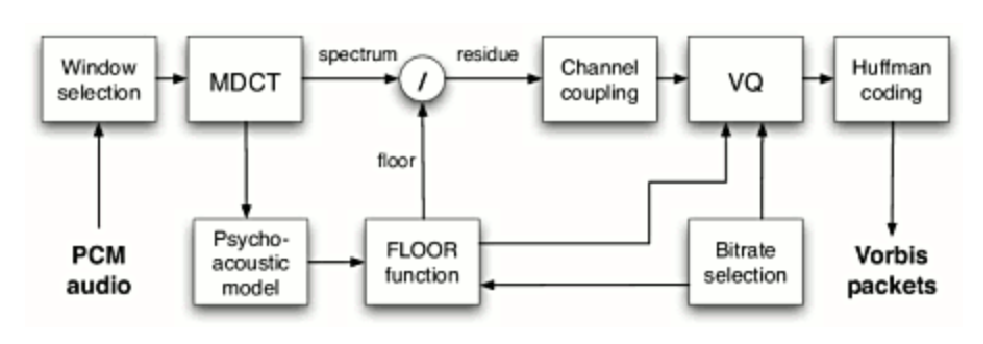
\includegraphics[keepaspectratio=true,scale=0.8]{figuras/algorithm.eps}
% 	\caption{Diagrama do algoritmo de compressão da Vorbis I \cite{algoritmocompressao}.}
% 	\label{algorithm}
% \end{figure}

\subsubsection{Estruturação}

O Vorbis é estruturado em pacotes e utiliza quatro tipos diferentes. O três primeiros tipos marcam três tipos diferentes de cabeçalho e devem estar dispostos na seguinte ordem: cabeçalho de identificação, cabeçalho de comentário e cabeçalho de configuração. Após os três pacotes de cabeçalho, todos os pacotes subsequentes são pacotes de áudio. E estrutura, de uma forma geral, é ilustrada na Figura \ref{vorbisstructure}.

\begin{figure}[ht]
	\centering
		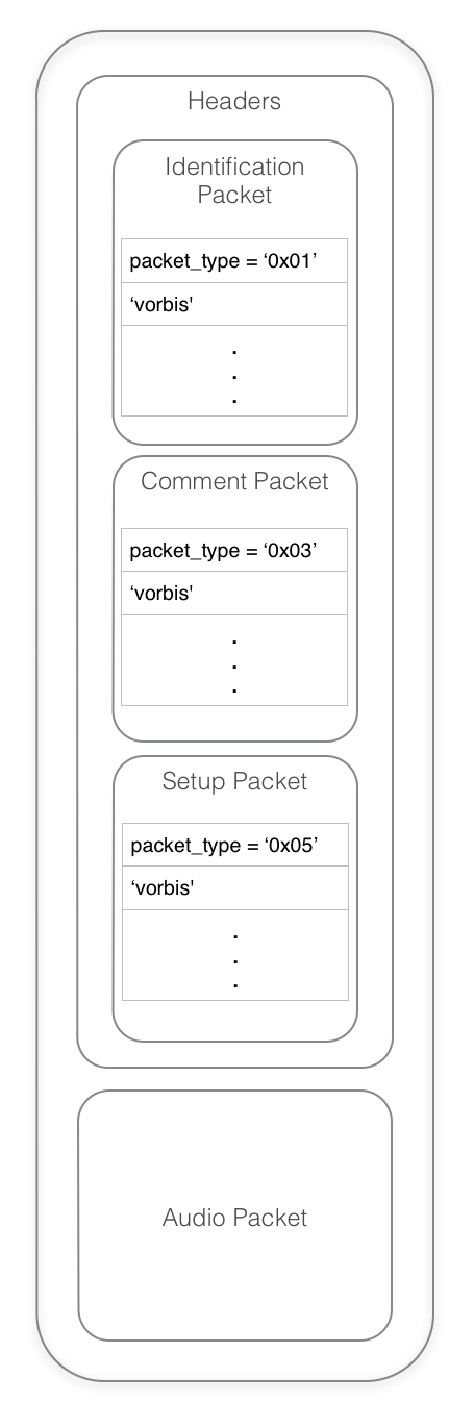
\includegraphics[keepaspectratio=true,scale=0.6]{figuras/vorbisstructure.eps}
	\caption{Diagrama Geral representando uma estrutura Vorbis.}
	\label{vorbisstructure}
\end{figure}

Todos os pacotes cabeçalhos começam com um byte para identificação do tipo de cabeçalho e mais seis bytes para identificação da \textit{string} ``vorbis''. O campos seguintes são específicos de cada pacote. O \textbf{\textit{identification packet}} identifica o fluxo de bits como Vorbis e contém informações sobre a versão do Vorbis usado, o número de canais de áudio e a taxa de amostragem. O segundo pacote é o \textbf{\textit{comment header}} e contém metadados que são comentários de usuários referentes ao pacote de áudio tais como nome da música, nome dos artistas ou o nome da gravadora. Este campo não é necessário para a decodificação do áudio, mas é um pacote obrigatório e deve ser identificado e ignorado adequamente para não corromper o arquivo. O Vorbis sugere alguns nomes de campos mas eles não são obrigatórios e outros também podem ser usados. A lista contém as seguintes sugestões: TITLE, VERSION, ALBUM, TRACKNUMBER, ARTIST, PERFORMER, COPYRIGHT, LICENSE, ORGANIZATION, DESCRIPTION, GENRE, DATE, LOCATION, CONTACT e ISRC. A maioria das informações necessárias para inicializar o decodificador estão contigas no \textit{\textbf{setup header}}. Ele contém informações de configuração do \textit{codec} e \textit{codebooks} contendo o VQ completo e o código de Huffman. Por último, temos o \textbf{\textit{audio packet}} que contém os dados de áudio do arquivo \cite{vorbis}.

No processo de decodificação, a primeira etapa da decodificação de pacotes de áudio é para ler e verificar o tipo de pacote. Um pacote não-audio quando um pacote de áudio é esperado indica corrupção de fluxo. O decodificador deve ignorar o pacote e não tentar decodificá-lo para áudio. Os pacotes de áudio começam com um único bit que precisa sempre ser 0 \cite{vorbis}.

\subsection{Licença de uso}

É intenção dos desenvolvedores Ogg Vorbis que o formato seja utilizável sem preocupações de propriedade intelectual e, por isso, são de domínio público. \textit{``Ogg Vorbis is a fully open, non-proprietary, patent-and-royalty-free (...)''} \cite{license}. O Ogg Vorbis está sob licença BSD e os termos de licença estão descritos e acessíveis em \cite{licenseterms}.

\section{Reuso de Requisitos}

Segundo \cite{sommerville2004software}, ``quando se desenvolve requisitos para um novo sistema, deve-se, na medida do possível, reutilizar os requisitos de outros sistemas que foram desenvolvidos para a mesma área da aplicação''. Para \cite{pabre}, o reuso de requisitos é ``a tendência de se utilizar o conhecimento adquirido em experiências anteriores no levantamento de requisitos e impulsionar a reutilização desse conhecimento''.

Por meio do método analítico, o reuso de requisitos é uma das técnicas conhecidas da atividade de elicitação de requisitos que visa analisar e estudar a viabilidade de reutilização de especificações existentes de sistemas legados ou sistema com funcionalidades de negócio similares. As principais vantagens do uso desta técnica são: melhorar a qualidade e elicitação de requisitos e reduzir o custo e tempo envolvidos no desenvolvimento do software visto que os requisitos reutilizados já foram analisados e validados em outros sistemas. Requisitos reutilizados são mais facilmente assimilados por usuários pois, de certa forma, já são conhecidos por eles \cite{brunobrum}.

\section{User Stories}

As \textit{User Stories} ou Histórias de Usuário apresentam algumas das características dos casos de usos ou das declarações tradicionais de requisitos e tem sido utilizada largamente em ambiente ágil \cite{cohn2004user}. No processo de levantamento de requisitos, a \textit{User Story} é usada como instrumento de escrita que descreve a especificação de uma funcionalidade do software em um cartão \cite{beck2001planning}. Um formato simples de \textit{user story} é sugerida por \cite{cohn2004user} e apresenta a seguite sintaxe: \textit{\textbf{Como um} tipo de usuário \textbf{eu quero} capacidade ou funcionalidade \textbf{de modo que} o valor do negócio ou benefício}. A Figura \ref{userstory} mostra um exemplo de cartão de \textit{user story}.

\begin{figure}[ht]
	\centering
		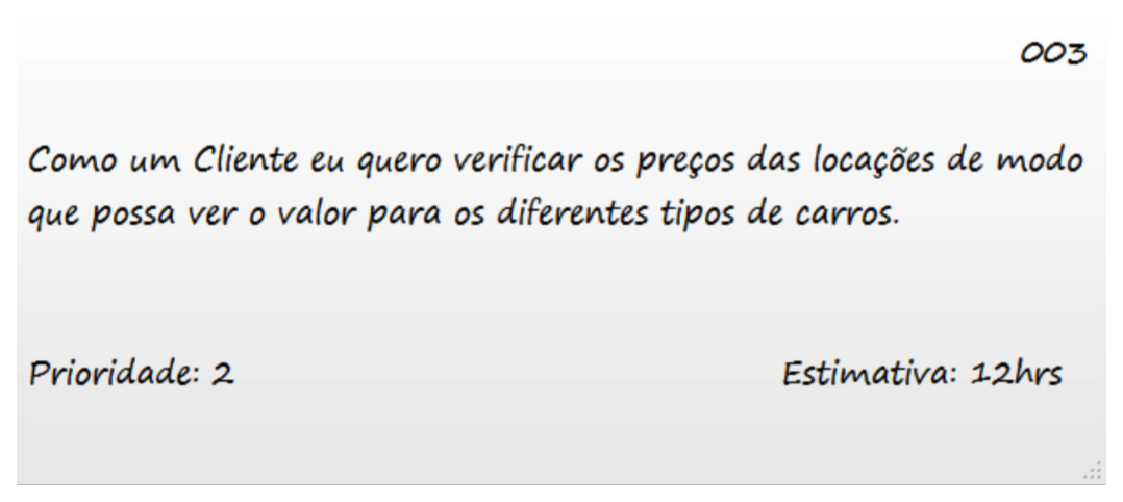
\includegraphics[keepaspectratio=true,scale=0.5]{figuras/userstory.eps}
	\caption{Um cartão de \textit{User Story}.}
	\label{userstory}
\end{figure}

Quando uma \textit{user story} é implementada, um teste de aceitação mais formal deverá ser escrito para assegurar que os objetivos da \textit{user story} sejam cumpridos. Os testes de aceitação são criados a partir de critérios de aceitação que são descritos no verso do cartão da \textit{user story}. Os critérios de aceitação define os limites de uma \textit{user story} e são utilizados para confirmar implementação da \textit{user story} e validar o seu correto funcionamento conforme o esperado \cite{cohn2004user}. A Figura \ref{criterio} mostra um exemplo de critério de aceitação.

\begin{figure}[ht]
	\centering
		\includegraphics[keepaspectratio=true,scale=0.5]{figuras/criterios.eps}
	\caption{Um cartão de Critérios de Aceitação.}
	\label{criterio}
\end{figure}

\cite{grenning2011test} observou que os textos em uma \textit{User Story} que descrevem os critérios de aceitação possuem os mesmo dados que um caso de uso. Mediante isso, o autor sugere que a história do usuário corresponde ao cenário do caso de uso principal, e que os testes de aceitação da história correspondem aos fluxos alternativos do caso de uso. Dando continuidade a explanação, \cite{grenning2011test} diz que os critérios de aceitação estão associados às histórias de usuário para especificar os requisitos de software que atendam as regras de negócio.







